\begin{frame}{}
    \LARGE Protein Design | \textbf{AlphaFold: Revolutionizing Protein Structure Prediction}
\end{frame}

\begin{frame}[allowframebreaks]{AlphaFold - A Brief History}
    \begin{figure}
        \centering
        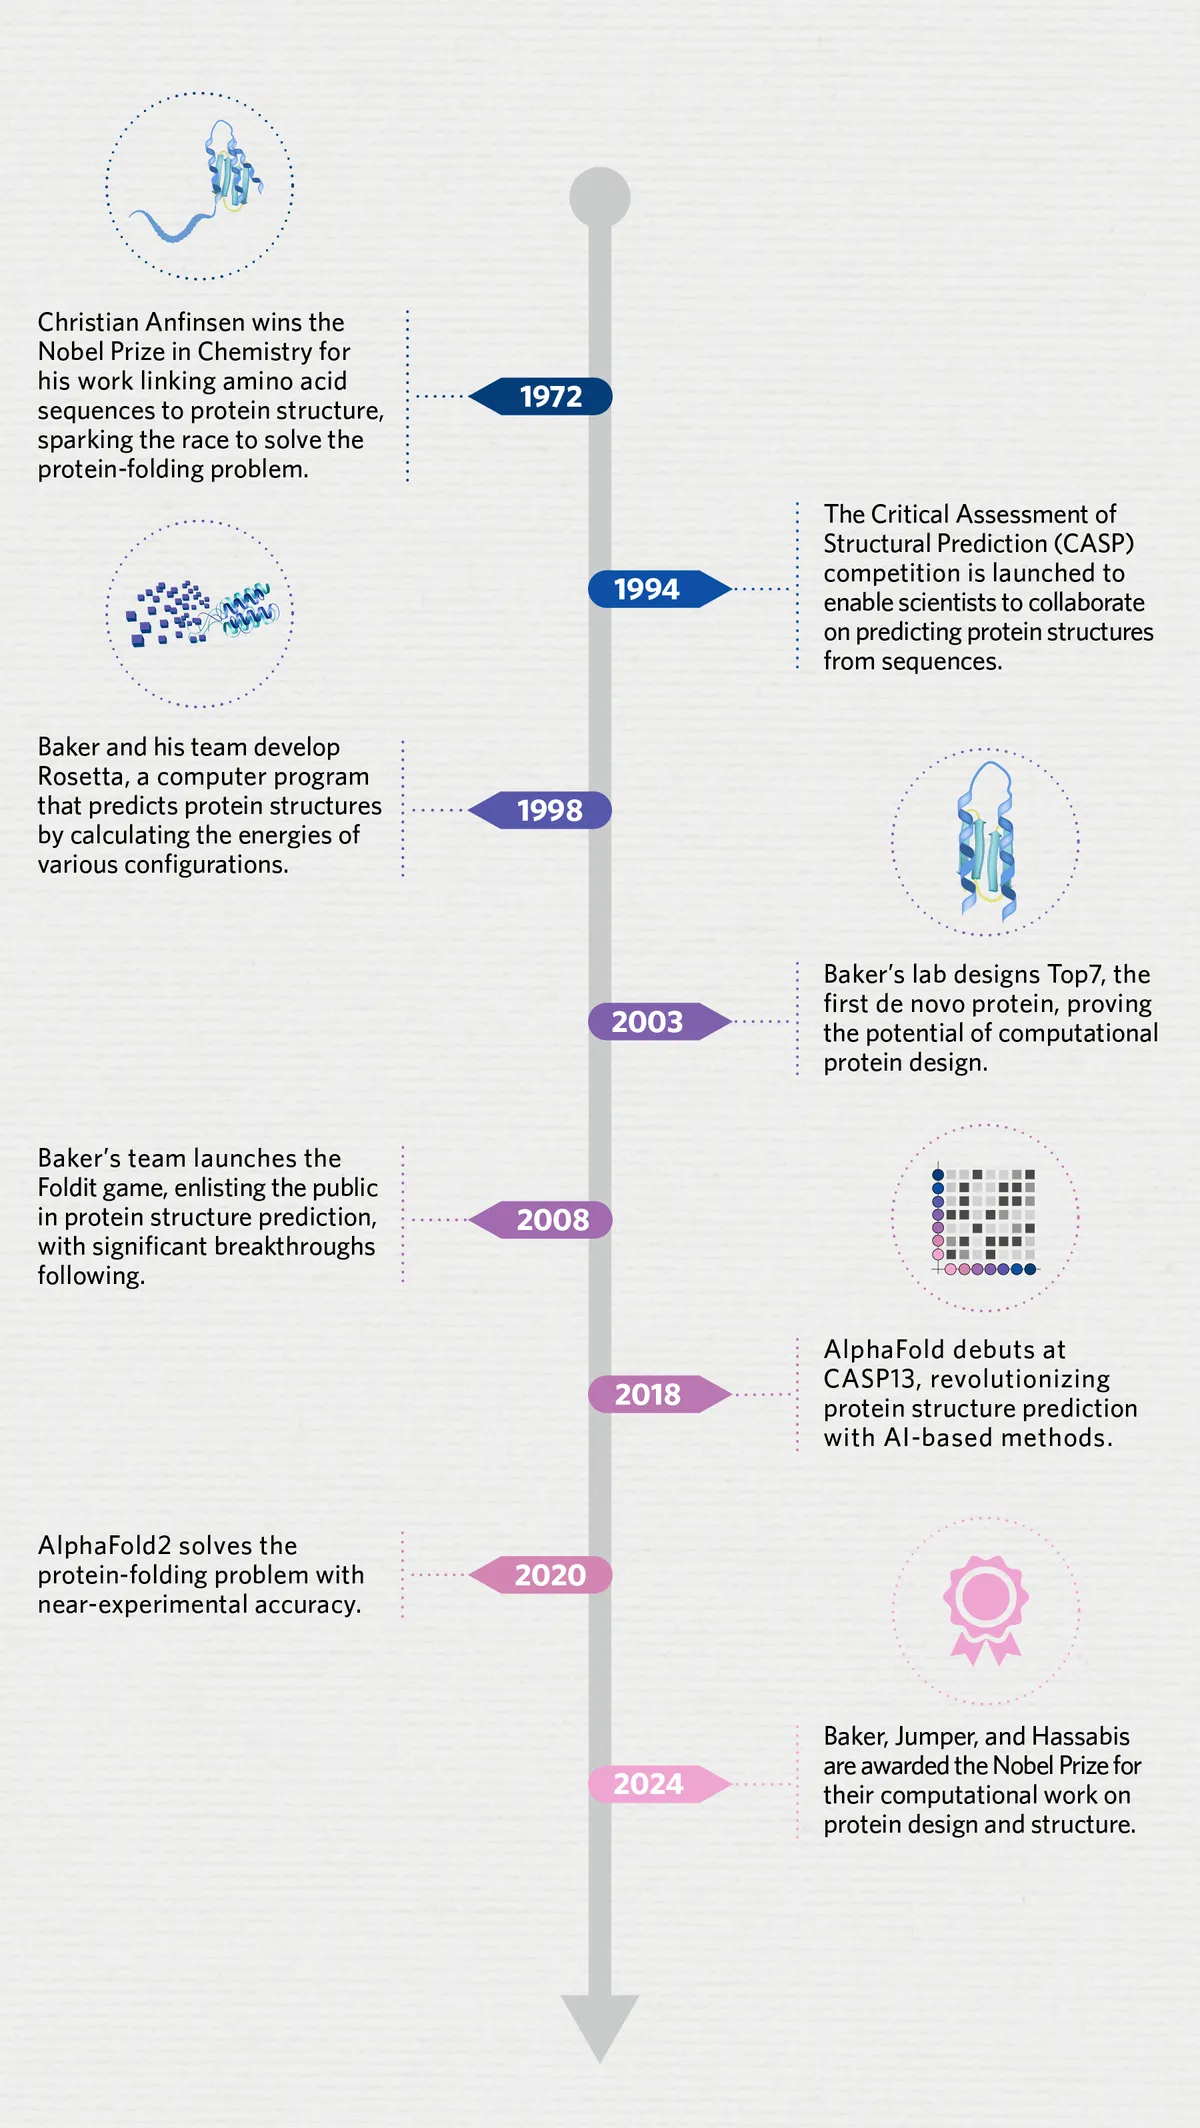
\includegraphics[angle=90,height=0.8\textheight,width=1\textwidth,keepaspectratio]{images/science/timeline.png}
        [Source: \href{https://www.the-scientist.com/the-journey-to-a-nobel-prize-a-protein-design-and-structure-research-timeline-72256}{TheScientist}]
    \end{figure}

    \framebreak

    \begin{figure}
        \centering
        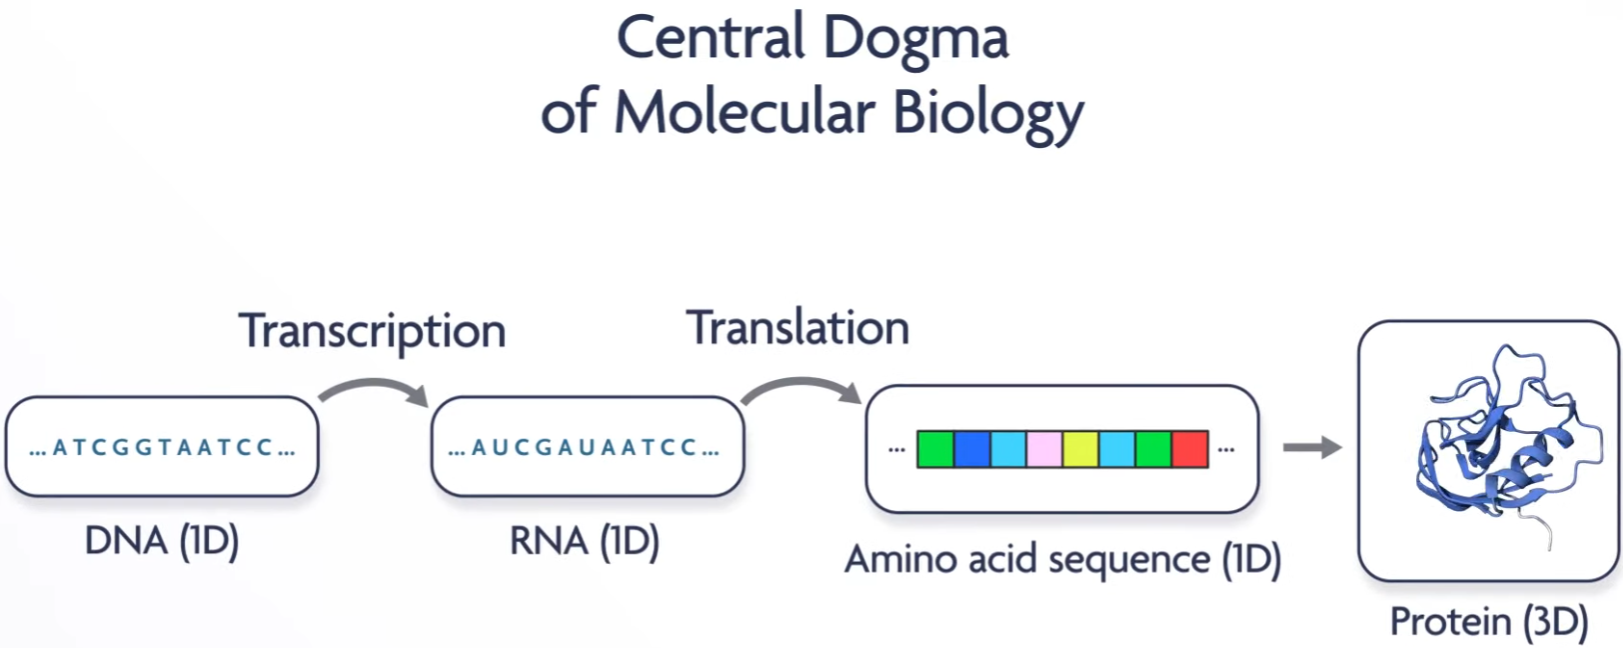
\includegraphics[height=0.6\textheight,width=1\textwidth,keepaspectratio]{images/science/central-dogma.png}
    \end{figure}
    
    \begin{itemize}
        \item DNA is transcribed into RNA, which is then translated into proteins.
        \item Proteins are made up of amino acids and fold into specific 3D structures.
        \item The structure of a protein determines its function in the cell.
    \end{itemize}

    \framebreak

    \begin{figure}
        \centering
        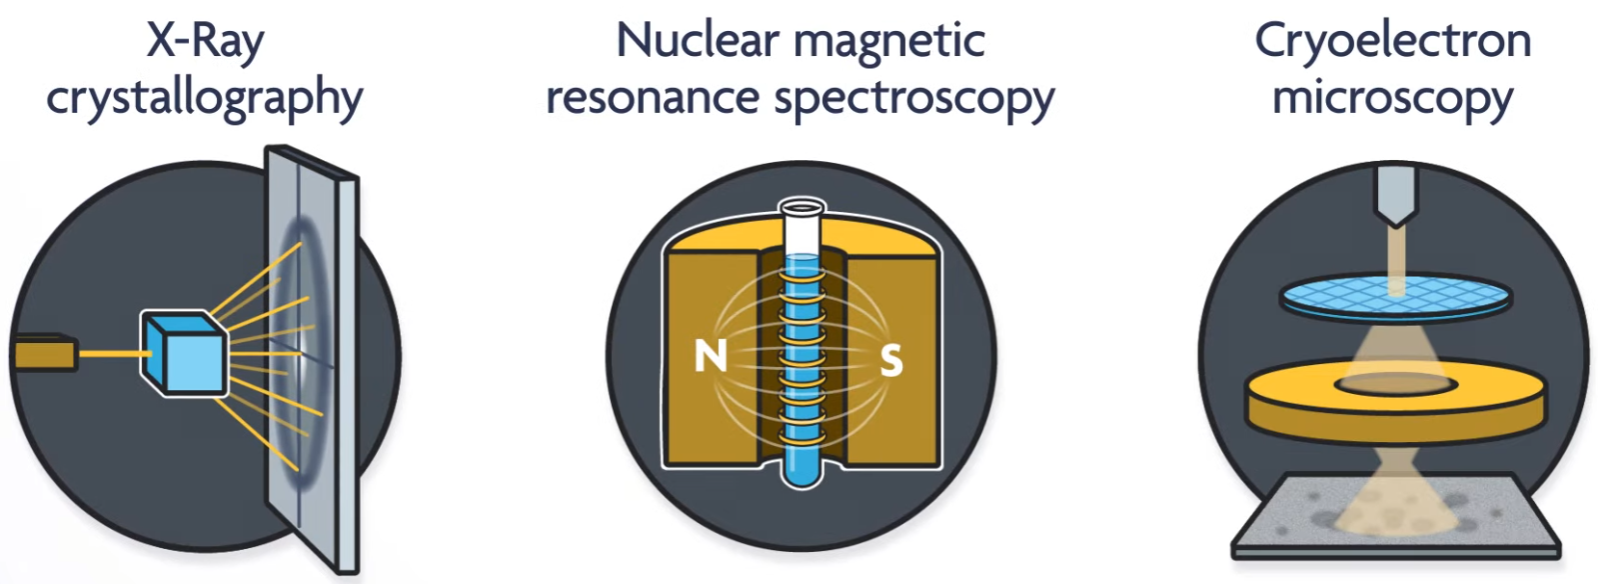
\includegraphics[height=0.6\textheight,width=1\textwidth,keepaspectratio]{images/science/traditional-method.png}
    \end{figure}

    \framebreak

    \begin{figure}
        \centering
        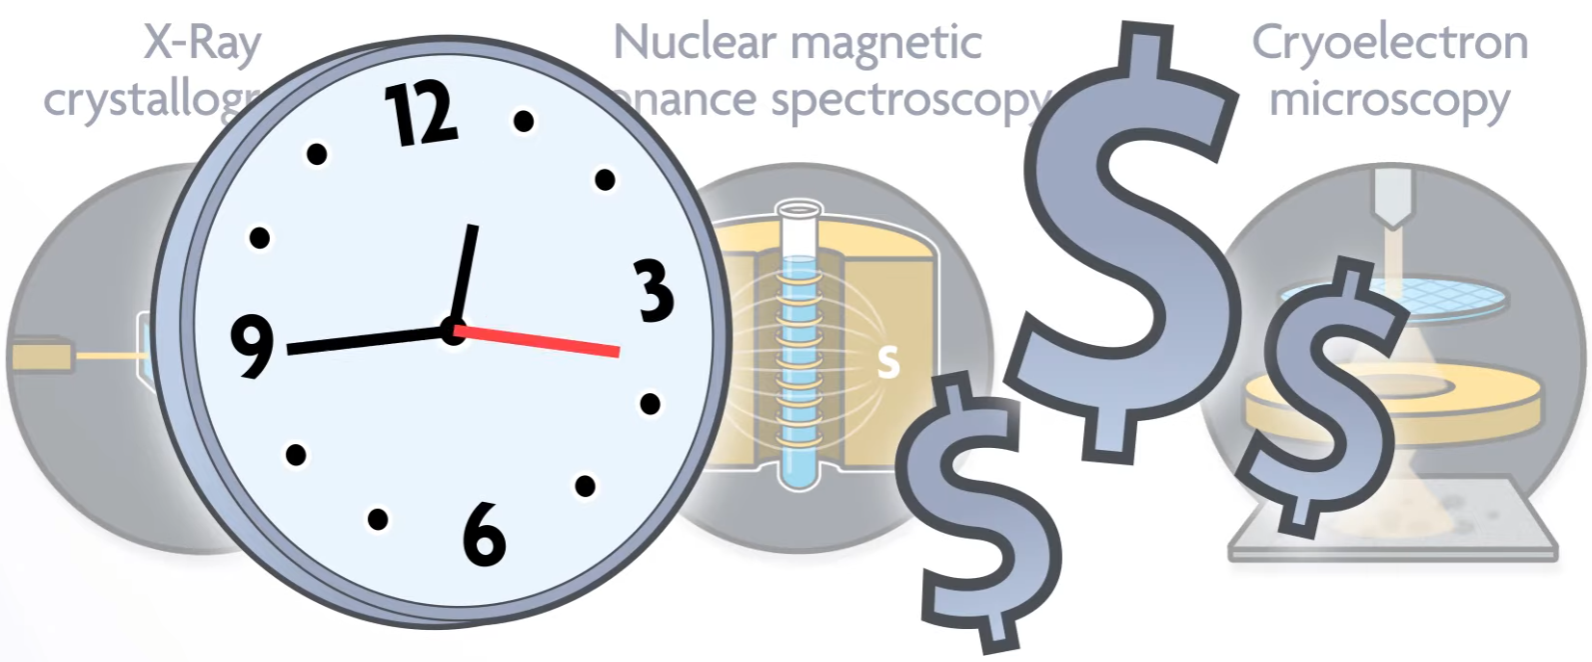
\includegraphics[height=0.6\textheight,width=1\textwidth,keepaspectratio]{images/science/traditional-method-limitation.png}
    \end{figure}
\end{frame}

\begin{frame}[allowframebreaks]{AlphaFold v1 (2018) - The Early Spark}
    \begin{figure}
        \centering
        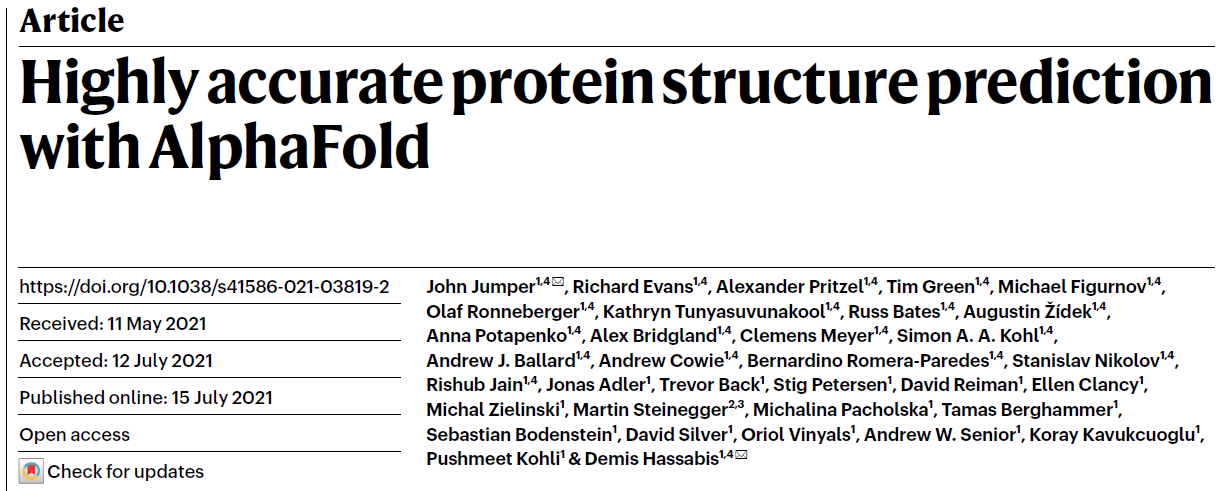
\includegraphics[width=\linewidth,height=0.9\textheight,keepaspectratio]{images/science/alphafold-1-paper.png}
    \end{figure}

    \framebreak
    
    \textbf{Motivation:}
    \begin{itemize}
        \item Predicting a protein's 3D shape from its amino acid sequence was a huge unsolved problem for decades.
        \item Scientists wanted a faster, more accurate way to figure out protein structures.
    \end{itemize}

    \textbf{Key Approach:}
    \begin{itemize}
        \item Looked for patterns in how amino acids change together across different proteins (co-evolution).
        \item Used neural networks to guess which amino acids are close to each other.
        \item Built 3D models by connecting these predicted contacts.
    \end{itemize}

    \framebreak

    \begin{figure}
        \centering
        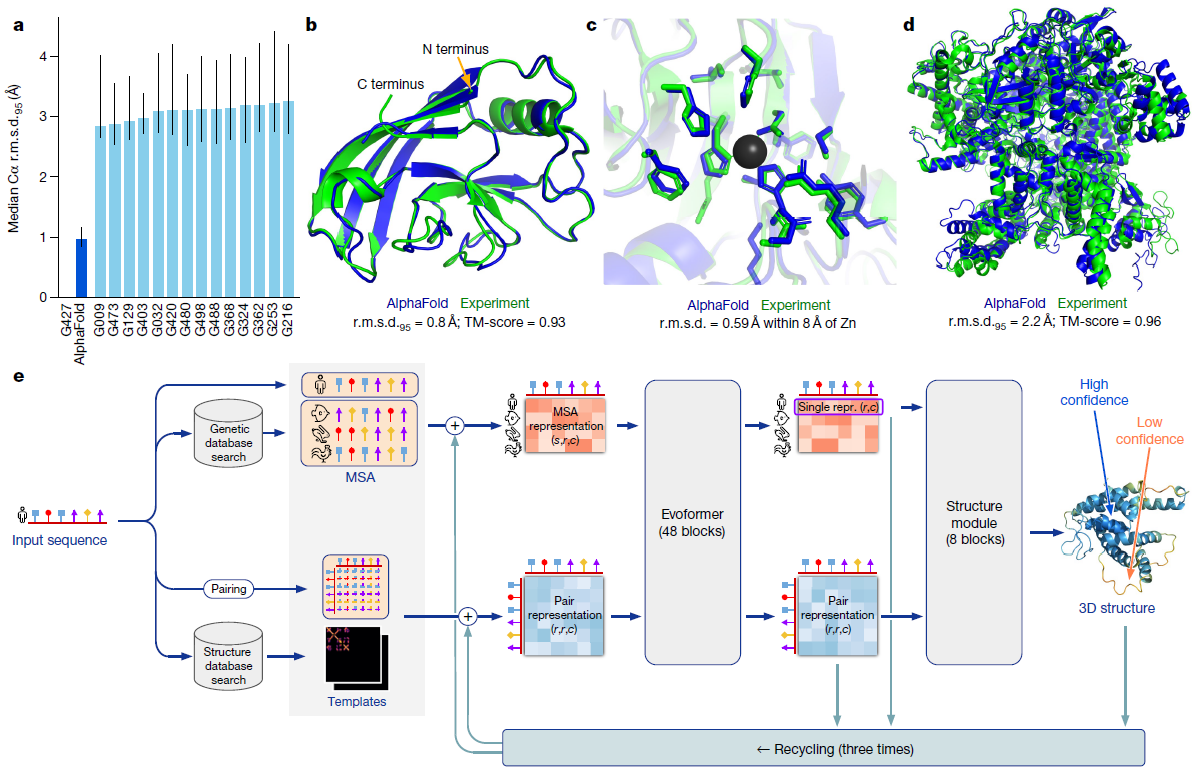
\includegraphics[width=\linewidth,height=0.85\textheight,keepaspectratio]{images/science/alphafold-1-architecture.png}
        \caption*{AlphaFold v1 Architecture: Neural networks predicting amino acid contacts.}
    \end{figure}
    
    \framebreak

    \begin{figure}
        \centering
        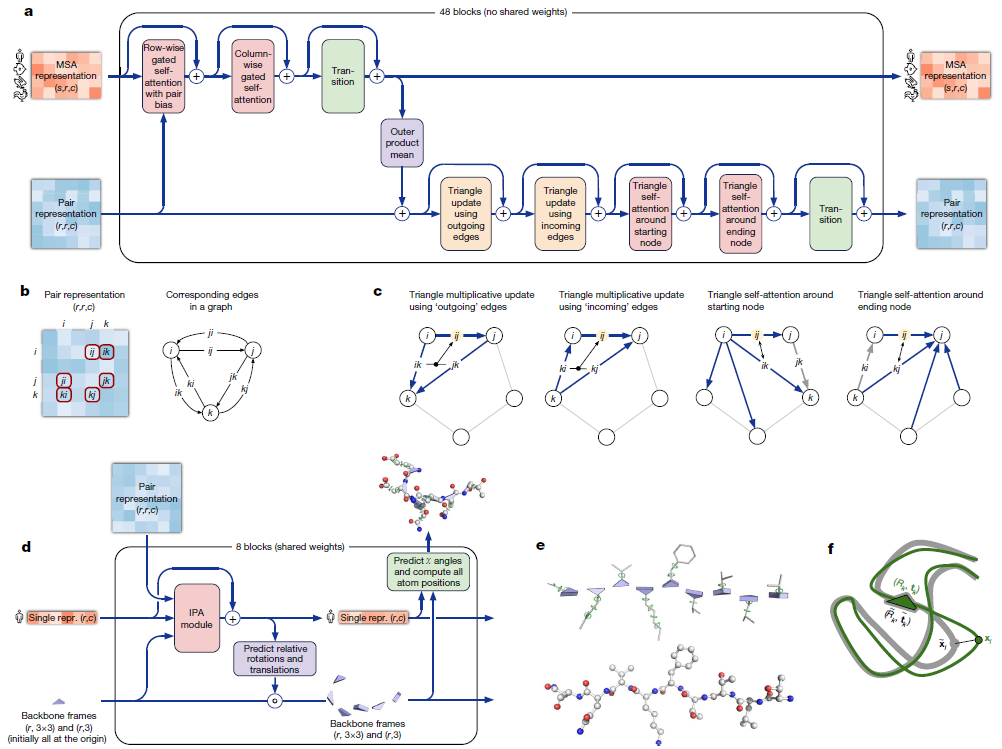
\includegraphics[width=\linewidth,height=0.85\textheight,keepaspectratio]{images/science/alphafold-1-architecture-2.png}
        \caption*{AlphaFold v1 Architecture Details.}
    \end{figure}
    
    \framebreak

    \begin{figure}
        \centering
        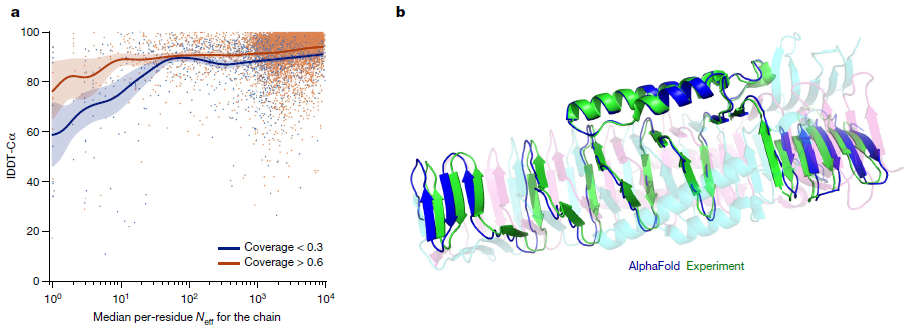
\includegraphics[width=\linewidth,height=0.85\textheight,keepaspectratio]{images/science/alphafold-1-msa-depth.png}
        \caption*{AlphaFold v1: Effect of MSA depth and cross-chain contacts.}
    \end{figure}
    
    \framebreak

    \textbf{Outcome:}
    \begin{itemize}
        \item AlphaFold v1 was the best performer in the CASP13 competition.
        \item Proved that AI could help solve the protein folding problem.
    \end{itemize}

    \textbf{Limitations:}
    \begin{itemize}
        \item Did not predict 3D structures directly—used contact maps as a middle step.
        \item Needed lots of evolutionary data to work well.
        \item Was less accurate than later versions.
    \end{itemize}
\end{frame}


\begin{frame}[allowframebreaks]{AlphaFold 2 (2020) - A Revolution}
    \begin{figure}
        \centering
        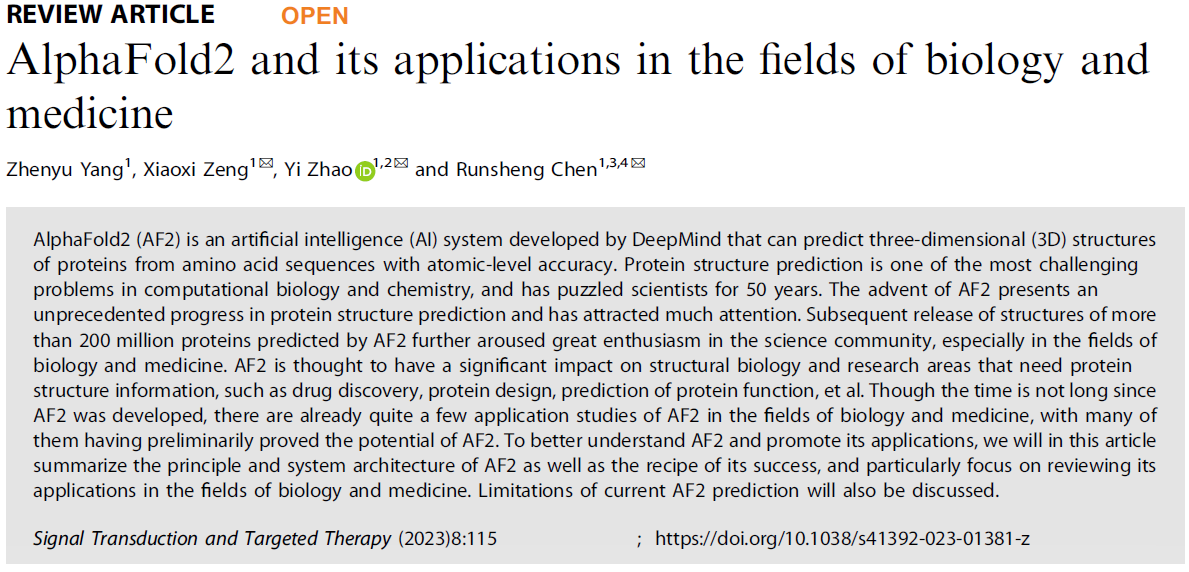
\includegraphics[width=\linewidth,height=0.9\textheight,keepaspectratio]{images/science/alphafold-2-paper.png}
    \end{figure}
    
    \framebreak

    \textbf{Why AlphaFold 2?}
    \begin{itemize}
        \item Scientists wanted a tool that was much faster and more accurate than before.
        \item The goal: Predict protein shapes quickly, with very high accuracy, and less manual work.
    \end{itemize}

    \textbf{How does it work?}
    \begin{itemize}
        \item Looks at lots of related protein sequences (MSA) and uses known structures as hints.
        \item Uses a special "Evoformer" module to find patterns in the data.
        \item Directly predicts the 3D positions of all atoms in the protein.
    \end{itemize}

    \framebreak

    \begin{figure}
        \centering
        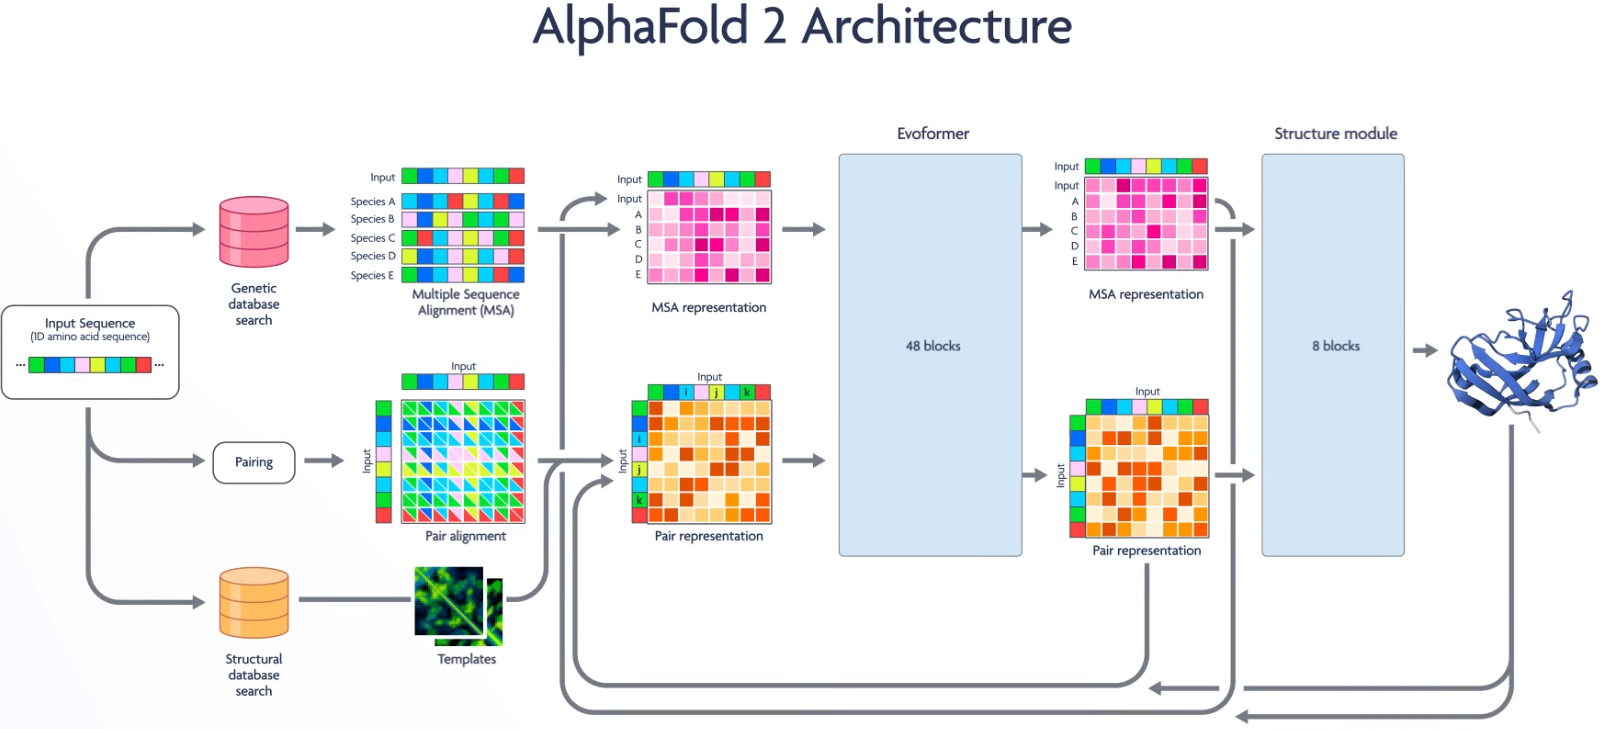
\includegraphics[width=\linewidth,height=0.85\textheight,keepaspectratio]{images/science/alphafold-2-architecture.png}
        \caption*{AlphaFold 2 Architecture: Directly predicts 3D coordinates from amino acid sequences.}
    \end{figure}

    \framebreak

    \begin{figure}
        \centering
        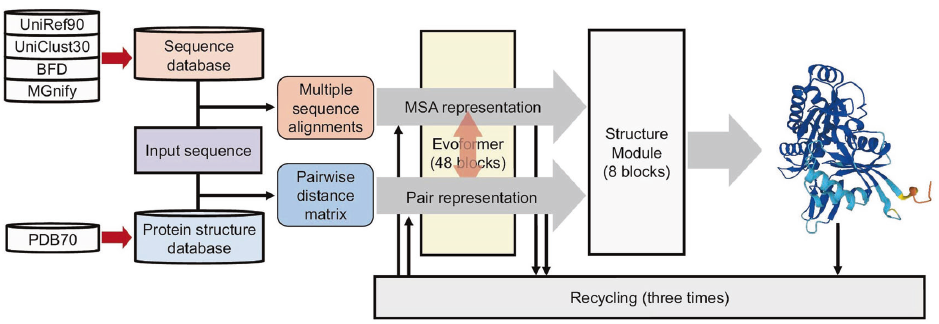
\includegraphics[width=\linewidth,height=0.85\textheight,keepaspectratio]{images/science/alphafold-2-application-1.png}
        \caption*{The overall architecture of AF2.}
    \end{figure}

    \framebreak

    \begin{figure}
        \centering
        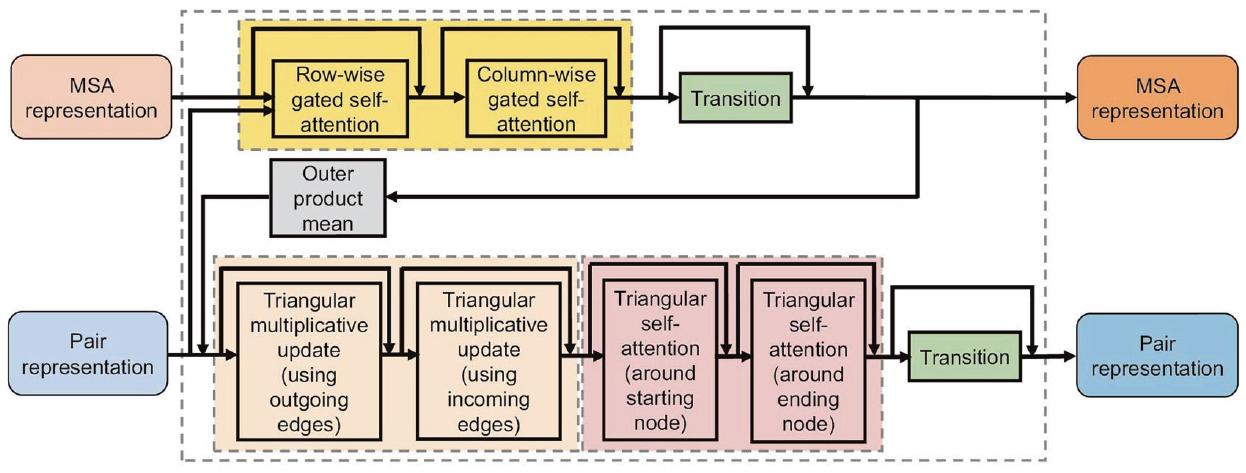
\includegraphics[width=\linewidth,height=0.85\textheight,keepaspectratio]{images/science/alphafold-2-application-2.png}
        \caption*{Components of a block in Evoformer.}
    \end{figure}

    \framebreak

    \begin{figure}
        \centering
        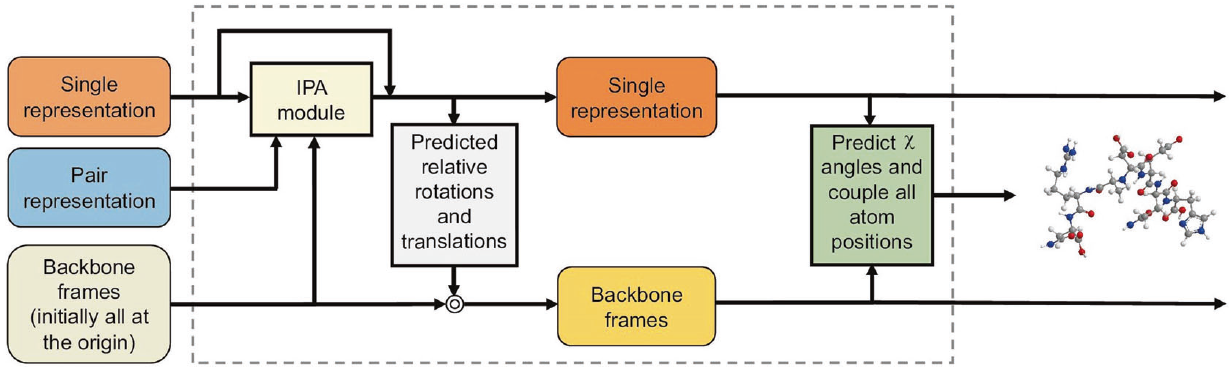
\includegraphics[width=\linewidth,height=0.85\textheight,keepaspectratio]{images/science/alphafold-2-application-3.png}
        \caption*{Components of a block in the structure module.}
    \end{figure}

    \framebreak

    \begin{figure}
        \centering
        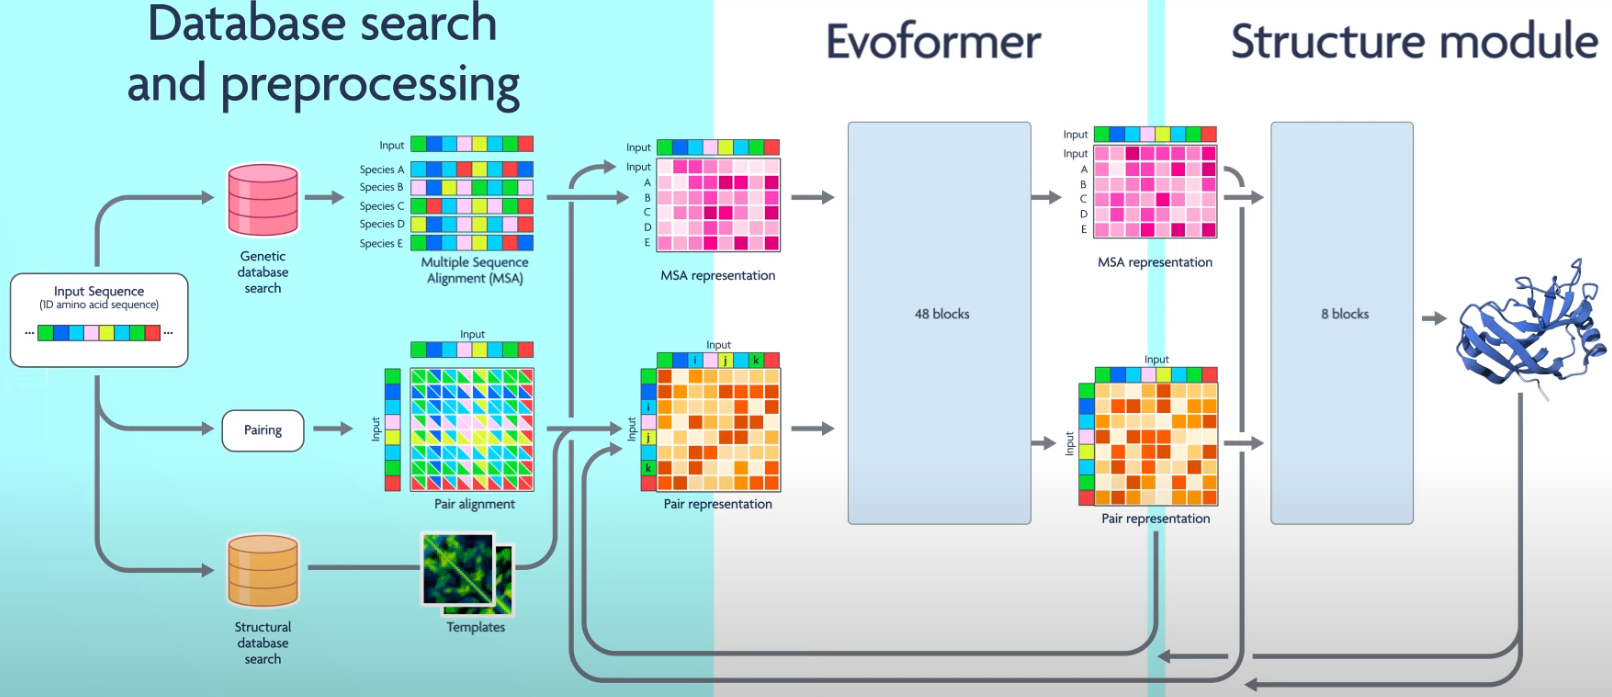
\includegraphics[width=\linewidth,height=0.85\textheight,keepaspectratio]{images/science/alphafold-2-architecture-2.png}
        \caption*{AlphaFold 2 Architecture: Directly predicts 3D coordinates from amino acid sequences.}
    \end{figure}

    \framebreak

    \textbf{How well did it do?}
    \begin{itemize}
        \item In the CASP14 competition, AlphaFold 2 was twice as accurate as any other method.
        \item It could predict protein shapes with errors as small as 1.5 Å (that’s really close!).
    \end{itemize}

    \framebreak

    \begin{figure}
        \centering
        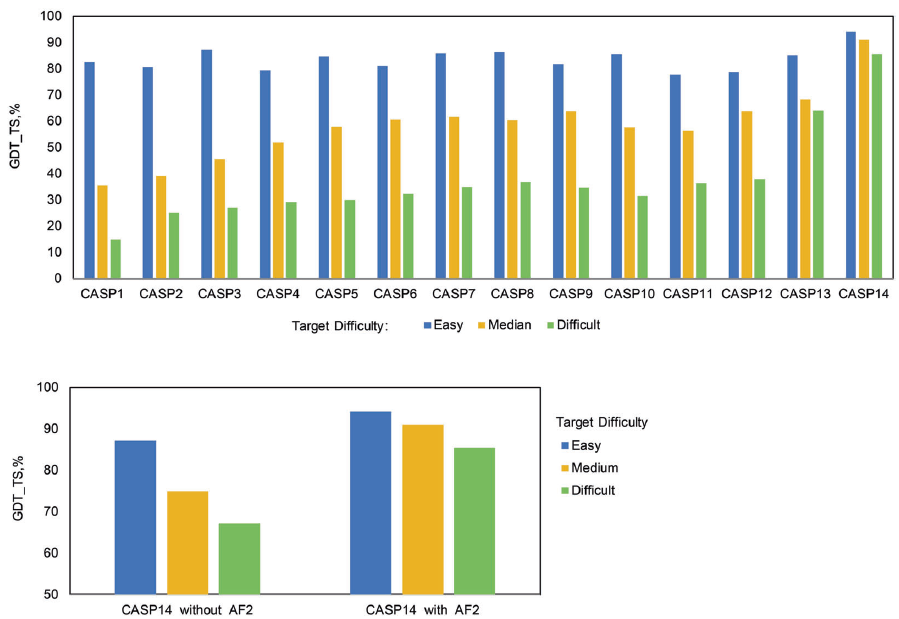
\includegraphics[width=\linewidth,height=0.8\textheight,keepaspectratio]{images/science/alphafold-2-result.png}
        \caption*{Performances of protein structure prediction indicated as backbone agreement with that of structures determined by experiments for
the best models in CASPs.}
    \end{figure}

    \framebreak

    \begin{figure}
        \centering
        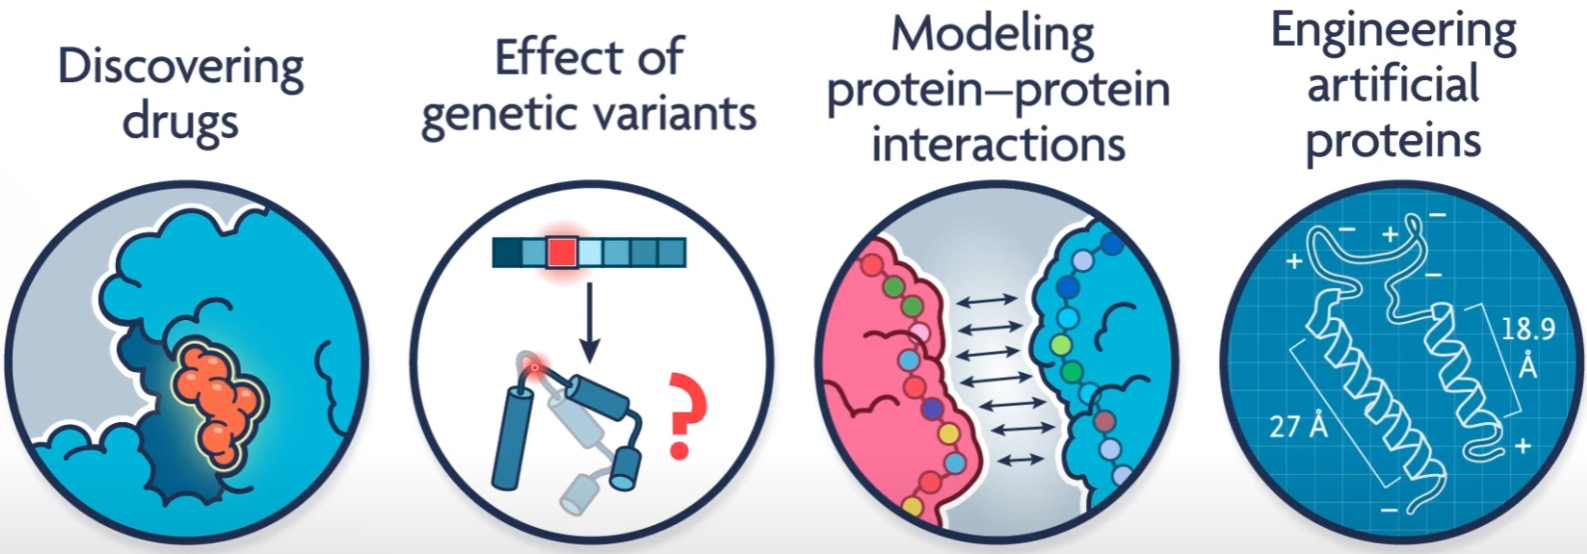
\includegraphics[width=\linewidth,height=0.85\textheight,keepaspectratio]{images/science/alphafold-2-applications.png}
        \caption*{Applications of AlphaFold 2.}
    \end{figure}

    \framebreak

    \textbf{What are its limits?}
    \begin{itemize}
        \item Works best for single protein chains, not big complexes.
        \item Has trouble with floppy or unusual protein regions.
    \end{itemize}
\end{frame}

\begin{frame}[allowframebreaks]{AlphaFold 3 (May 2024) – All Molecules Under One Roof}
    \begin{figure}
        \centering
        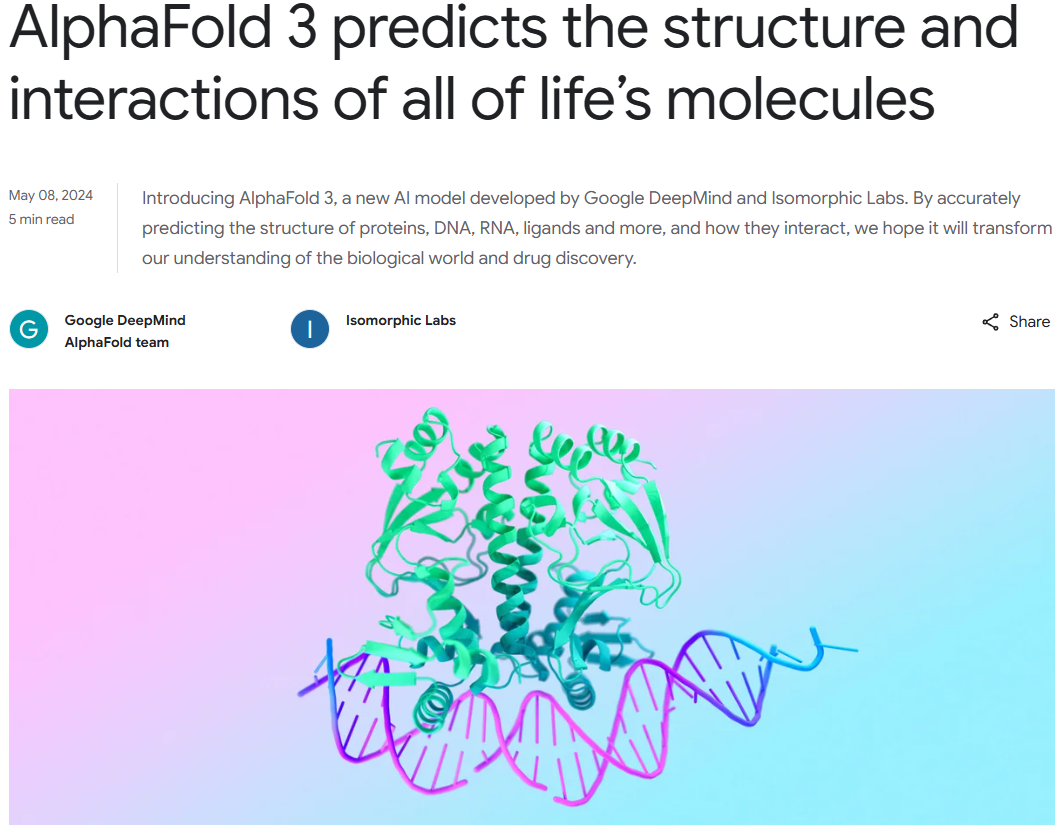
\includegraphics[width=\linewidth,height=0.9\textheight,keepaspectratio]{images/science/alphafold-3-paper.png}
        [Source: \href{https://blog.google/technology/ai/google-deepmind-isomorphic-alphafold-3-ai-model/}{Google}]
    \end{figure}

    \framebreak

    \textbf{Why AlphaFold 3?}
    \begin{itemize}
        \item Scientists wanted to predict not just proteins, but also DNA, RNA, and small molecules.
        \item Needed a tool to see how all these molecules interact together.
    \end{itemize}

    \textbf{What's new in AlphaFold 3?}
    \begin{itemize}
        \item Uses a new "Pairformer" module to better understand how pairs of molecules interact.
        \item Adds a diffusion-based step to build 3D shapes of molecules.
        \item Can handle proteins, DNA, RNA, small molecules, and ions—all in one model.
    \end{itemize}

    \framebreak

    \begin{figure}
        \centering
        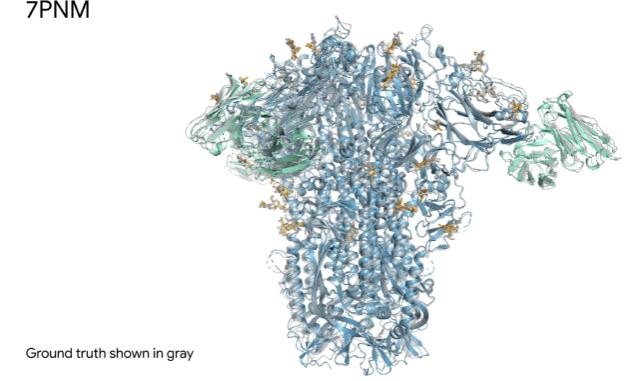
\includegraphics[width=\linewidth,height=0.8\textheight,keepaspectratio]{images/science/alphafold-3-protein.png}
    \end{figure}
    [Source: \href{https://blog.google/technology/ai/google-deepmind-isomorphic-alphafold-3-ai-model/}{Google}]

    \framebreak

    \begin{figure}
        \centering
        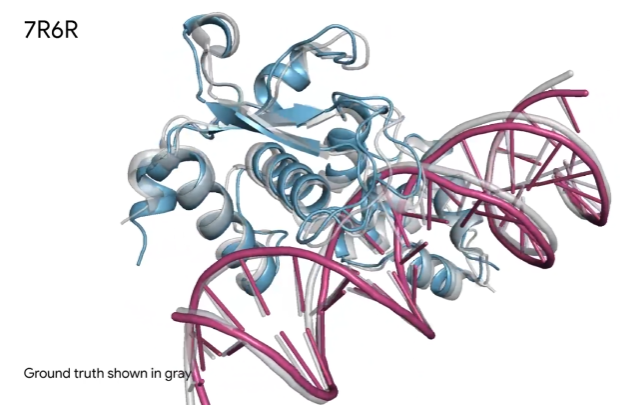
\includegraphics[width=\linewidth,height=0.8\textheight,keepaspectratio]{images/science/alphafold-3-7r6r.png}
    \end{figure}
    [Source: \href{https://blog.google/technology/ai/google-deepmind-isomorphic-alphafold-3-ai-model/}{Google}]

    \framebreak

    \textbf{What can it do?}
    \begin{itemize}
        \item Predicts how different types of molecules fit and work together.
        \item Helps study big molecular machines made of many parts.
    \end{itemize}

    \textbf{How can you use it?}
    \begin{itemize}
        \item Free public server for researchers (up to 20 predictions per day).
        \item Commercial access available for companies.
    \end{itemize}

    \framebreak

    \begin{figure}
        \centering
        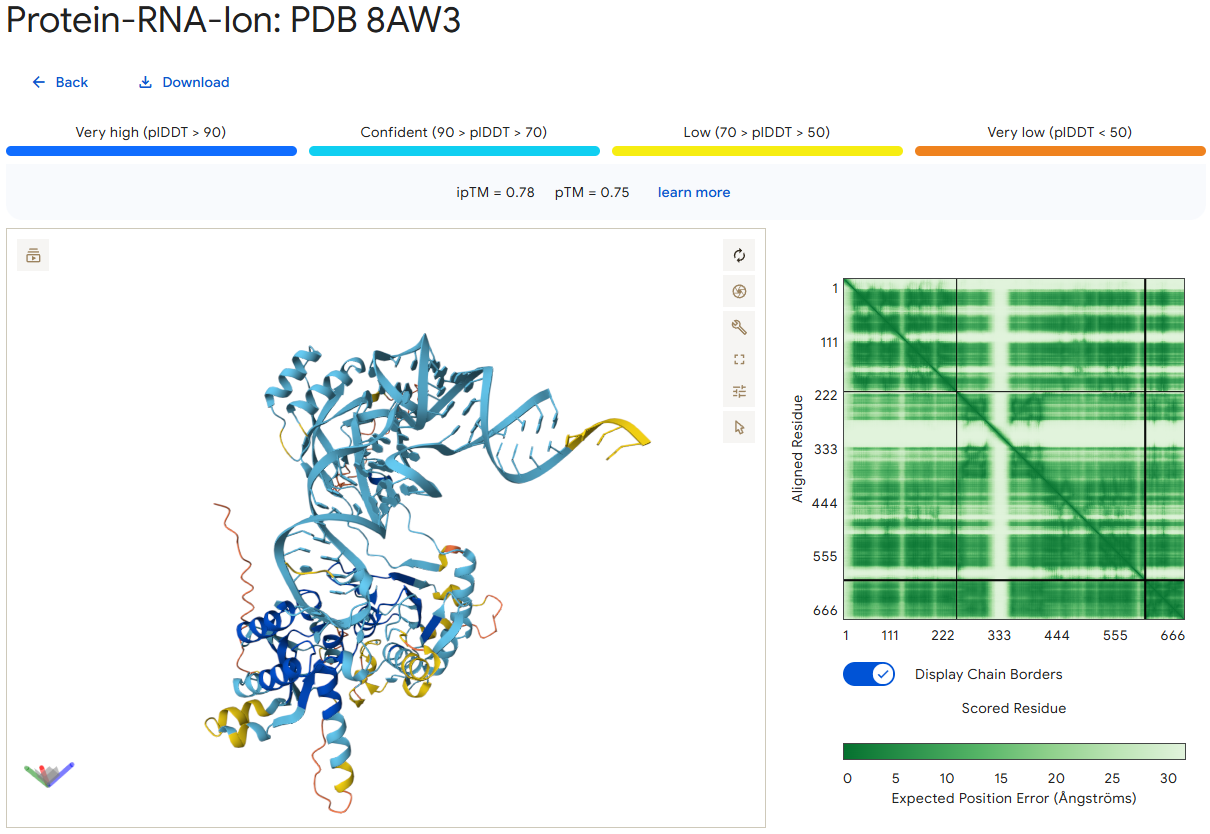
\includegraphics[width=\linewidth,height=0.8\textheight,keepaspectratio]{images/science/alphafold-3-playground-1.png}
    \end{figure}
    [Playground: \href{https://alphafoldserver.com/example/examplefold_pdb_8aw3}{Protein-RNA-Ion: PDB 8AW3}]

    \framebreak

    \begin{figure}
        \centering
        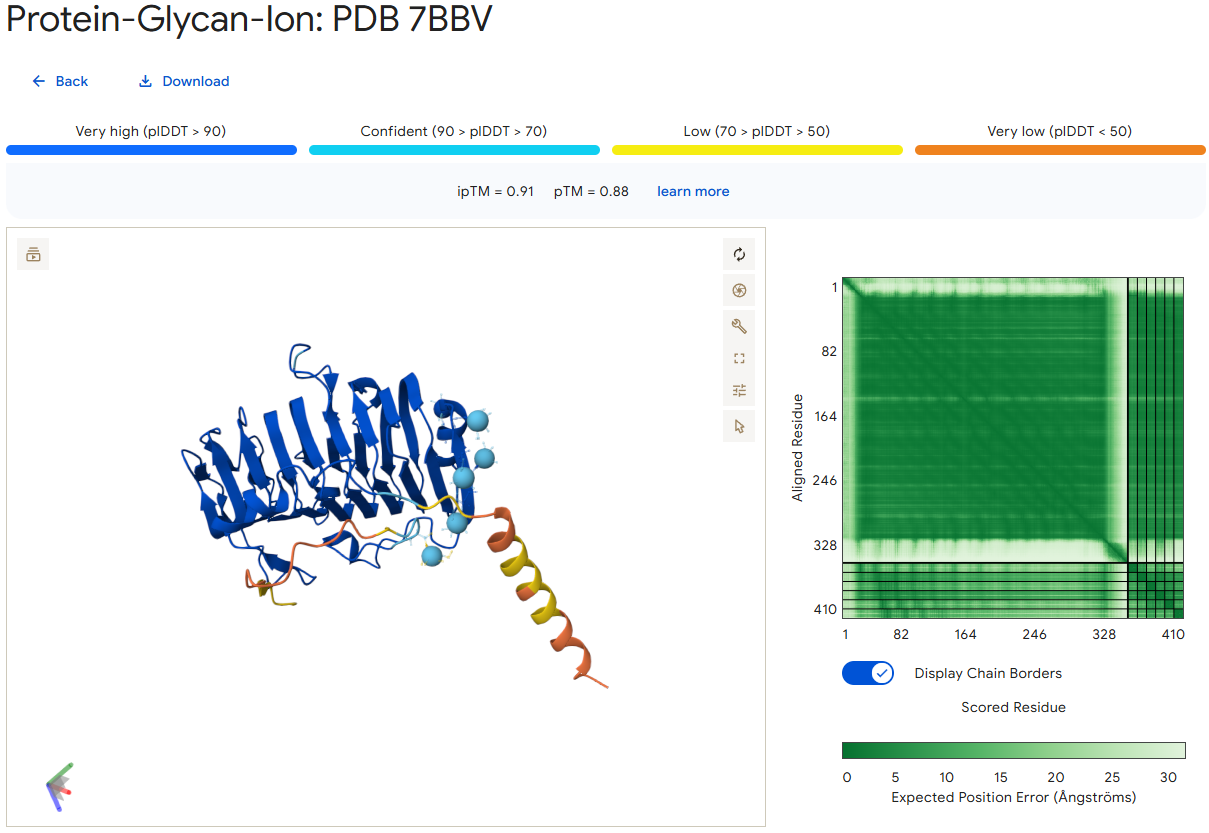
\includegraphics[width=\linewidth,height=0.8\textheight,keepaspectratio]{images/science/alphafold-3-playground-2.png}
    \end{figure}
    [Playground: \href{https://alphafoldserver.com/example/examplefold_pdb_7bbv}{Protein-Glycan-Ion: PDB 7BBV}]

    \framebreak

    \begin{figure}
        \centering
        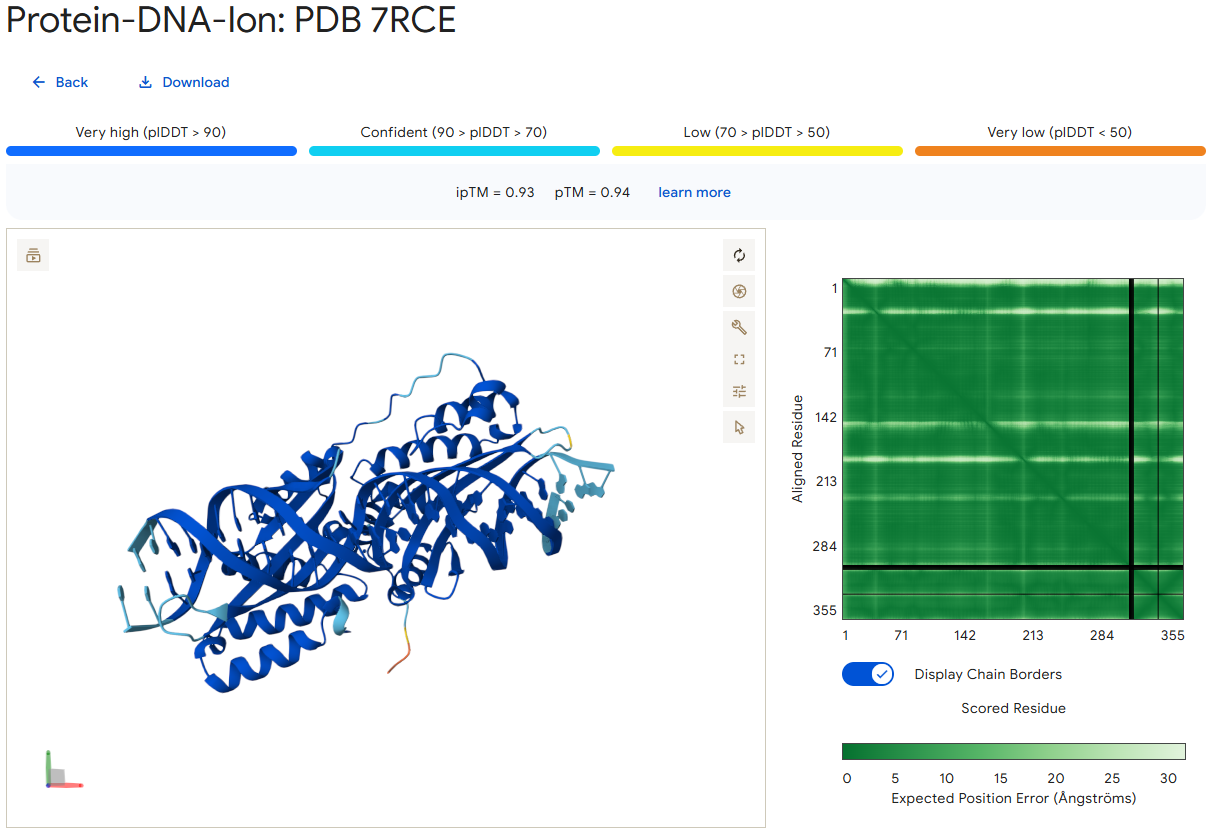
\includegraphics[width=\linewidth,height=0.8\textheight,keepaspectratio]{images/science/alphafold-3-playground-3.png}
    \end{figure}
    [Playground: \href{https://alphafoldserver.com/example/examplefold_pdb_7rce}{Protein-DNA-Ion: PDB 7RCE}]
\end{frame}

% \begin{frame}[allowframebreaks]{AlphaFold: Key Features and Impact}
% \begin{itemize}
%     \item AlphaFold is a generative AI model that predicts protein structures from amino acid sequences.
%     \item It uses deep learning to understand the complex relationships between amino acids.
%     \item The model was trained on a large dataset of known protein structures.
%     \item AlphaFold achieved unprecedented accuracy in the Critical Assessment of protein Structure Prediction (CASP) competition.
%     \item It can predict the 3D structure of proteins in a matter of hours, a task that previously took months or years.
% \end{itemize}
% \framebreak
% \begin{figure}
%     \centering
%     \includegraphics[width=0.8\linewidth,height=0.7\textheight,keepaspectratio]{images/science/alphafold.png}
%     \caption{AlphaFold's predicted structure of a protein.}
% \end{figure}
% \framebreak
% \textbf{Applications of AlphaFold}
% \begin{itemize}
%     \item Drug discovery: Helps identify potential drug targets by understanding protein interactions.
%     \item Disease research: Aids in understanding diseases caused by protein misfolding, like Alzheimer's.
%     \item Synthetic biology: Assists in designing new proteins with specific functions.
%     \item Environmental science: Helps in understanding proteins involved in biogeochemical cycles.
% \end{itemize}
% \framebreak
% \textbf{Limitations and Challenges}
% \begin{itemize}
%     \item AlphaFold's predictions are based on existing data, so it may struggle with novel protein folds.
%     \item It does not predict protein dynamics or interactions with other molecules.
%     \item The model requires significant computational resources, which may not be accessible to all researchers.
%     \item Ethical considerations: The potential misuse of protein design for harmful purposes.
% \end{itemize}
% \end{frame}